\chapter{Experiments} \label{chp:experiments}
\section{Suppression Task} \label{sec:sup}
\subsection{Intuitive Overview} \label{ssec:sup_intuition}
The Suppression Task refers to an experiment conducted by \cite{byrne1989suppressing} and is a classical example of the inadequacy of monotonic logics for modelling human reasoning. In classical logic, if our knowledge base $kb$ is such that $kb \models \phi$, then it must be the case that $kb \cup \psi \models \phi$. However, in the suppression task participants no longer draw classically valid inferences when new information is added. The task is often formulated as follows:

\begin{itemize}
\item $e \rightarrow l$: If she has an essay to write ($e$), she will study late in the library ($l$).
\item $\top \rightarrow e$: She has an essay to write ($e$).
\item $o\rightarrow l$: If the library is open ($o$), she will study late in the library ($l$).
\end{itemize}

Given only the rules $(e \rightarrow l)$ and $(\top \rightarrow e)$, the participants consistently concluded that she would study late in the library, seemingly drawing the classical logic inference $\frac{e \rightarrow l, e}{l}$ with \textit{modus ponens}. But when given the additional rule $o\rightarrow l$, participants no longer believe that they have enough information to judge whether she will study late in the library, and a significant portion of them no longer draw the classical conclusion. This effect, called Suppression, demonstrates the need for something more than classical logic for modelling human reasoning.

\subsection{Modelling the Suppression Task} \label{ssec:sup_mod}
Work by \cite{dietz2014modeling} has shown that the WCS is an adequate non-monotonic logic for modelling the Suppression Task. Under the WCS and \L ukasiewicz 3-valued logic the task is usually modelled as follows for the case without suppression:
\begin{enumerate}
\item Initial logic program: $P = \{e \rightarrow l, \top \rightarrow e \}$. This program represents the task without information about what happens if the library is open.
\item Addition of Abnormality: $P = \{e \land \lnot ab_1 \rightarrow l, \top \rightarrow e, \bot \rightarrow ab_1 \}$. The program now reflects the possibility that some abnormal event may prevent her from going to the library, but because we have no information about the nature of this event, it is set to false by default.
\item Weak Completion: $wc(P) = \{e \land \lnot ab_1 \leftrightarrow l, \top \leftrightarrow e, \bot \leftrightarrow ab_1 \}$. Weak completion is applied to the logic program and, in this case, only implications need to be changed to bijections.
\item Semantic Operator:
\begin{itemize}
\item Execution 1: $\top=\{e\}, \bot=\{ab_1\}$
\item Execution 2: $\top=\{e,l\}, \bot=\{ab_1\}$
\end{itemize}
\end{enumerate}

After application of the semantic operator $l$ is true in the least model, and so participants conclude that she will study late in the library (as when $P$ is evaluated classically). However, in the case where Suppression is observed, the same process yields a different result because of the presence of the extra conditional ($o\rightarrow l$).
\begin{enumerate}
\item Initial logic program: $P = \{e \rightarrow l, \top \rightarrow e, o \rightarrow l \}$. The initial program now includes information about the extra (suppressing) conditional.
\item Addition of Abnormality: $P = \{e \land \lnot ab_1 \rightarrow l, o \land \lnot ab_2 \rightarrow l, \top \rightarrow e, \lnot o \rightarrow ab_1, \lnot e \rightarrow ab_2 \}$. An abnormality $ab_i$ is an addition to an inference which captures the idea that external factors may invalidate the conclusion of the original inference. Adding abnormalities is a poorly described process and often relies on intuitionist views of what actually constitutes an abnormal situation. In this case we adopt the practise of identifying abnormalities as described in Appendix~\ref{ssec:addAbnormalities}.
\item Weak Completion: $wc(P) = \{((e \land \lnot ab_1) \lor (o \land \lnot ab_2)) \leftrightarrow l, \top \leftrightarrow e, \lnot o \leftrightarrow ab_1, \lnot e \leftrightarrow ab_2 \}$. Weak completion is applied to the logic program, combining rules with shared heads and replacing implications with bijections.
\item Semantic Operator:
\begin{itemize}
\item Execution 1: $\top=\{e\}, \bot=\{ab_2\}$
\end{itemize}
\end{enumerate}

Now suppression has been displayed in the logic program and the variable $l$ remains unknown in the least model.

\section{Wason Selection Task}
\subsection{Intuitive Overview} \label{ssec:wst_intuition}
\begin{table}
\begin{center}


\begin{tabular}{ c c c c c}
  & \textbf{$p$} & \textbf{$pq$} & \textbf{$pq\bar{q}$} & \textbf{$p\bar{q}$}\\ 
 Abstract & 36 & 39 & 5 & 19\\  
 Everyday & 23 & 37 & 11 & 29\\  
 Deontic & 13 & 19 & 4 & 64
\end{tabular}
\caption{The canonical results of the Wason Selection Task}
\label{tbl:can}
\end{center}
\end{table}


Another widely studied task in the psychological literature is the Wason Selection Task (WST), which asks participants to draw conclusions about which variables are able to falsify a given rule (\textit{Modus Tolens}\footnote{If $a\rightarrow b$, then $\lnot b \rightarrow \lnot a$}). We will look at this task in terms of the Abstract case of the task \citep{wason1968reasoning}. Each case is identical to each other in terms of classical logic representation, but each is interpreted differently by subjects. The WST is often used to illustrate that humans do no follow classical logic.

\subsection{Modelling the Wason Selection Task} \label{ssec:wst_mod}

\subsubsection*{Abstract Case}

\begin{figure}
\begin{center}
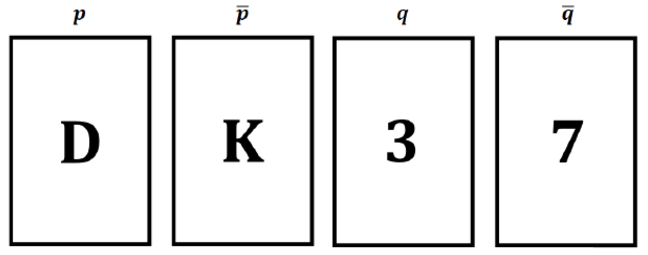
\includegraphics[scale=0.5]{wasonAbstract}
\caption{The Abstract case of the Wason Selection Task}
\end{center}
\end{figure}

The Abstract case of the WST presents the subject with four cards on a table. Their face-up sides read $D, K, 3,$ and $7$. They are asked which cards must be turned over to test the rule:

\begin{center}
``If there is a $D$ on one side of the card, then the other side shows $3$."
\end{center} 
Using classical logic, it is easy to see that turning $D$ to find anything but $3$ would invalidate the rule, as would turning $7$ and finding a $D$. Thus these two cards must be turned to check the rule. However, human subjects very seldom choose this classical answer set and instead overwhelmingly prefer to turn $D$ and $3$. Table~\ref{tbl:can} shows the most common card selection sets for participants.

A great many cognitive theories have been applied to these results, with varying degrees of success \cite{ragni2017formal}. This paper will focus on the WCS interpretation of the task provided by \citep{ragni2017wason}. This approach assumed an initial knowledge base containing only the rule $3 \leftarrow D$.

To illustrate this interpretation of the task we shall use the WCS to examine each of the four cards individually and see what conclusions can be drawn.

When $D$ is observed:

\[
KB = \{3 \leftarrow D, D\leftarrow \top \}
\]

However, at this point, the authors introduce the concept of an abnormality as discussed in \citep{ragni2017formal}. Now, the rule holds only provided that some abnormal even does not occur.

\[
KB_D = \{3 \leftarrow D \land \lnot ab_1, D \leftarrow \top, ab \leftarrow \bot \}
\]

\[
wcKB_D = \{3 \leftrightarrow D \land \lnot ab_1, D \leftrightarrow \top, ab \leftrightarrow \bot \}
\]

The authors also require that, to validate the rule, it must be evaluated after the semantic operator is iterated. Table~\ref{tbl:dcard} shows the result of repeatedly applying the semantic operator to $KB_D$. 

\begin{table}
\begin{center}

\begin{tabular}{ c c c }
 \textbf{Iteration} & \textbf{$\top$} & \textbf{$\bot$} \\ 
 0 &  &  \\  
 1 &  $D$ & $ab$  \\  
 2 &  $D$, $3$ & $ab$  
\end{tabular}
\caption{Applying the Weak Completion Semantics to the $D$ card of the WST.}
\label{tbl:dcard}

\end{center}
\end{table}

When the $K$ card is observed:

\[
KB_K = \{3 \leftarrow D \land \lnot ab_1, K \leftarrow \top, ab \leftarrow \bot \}
\]

\[
wcKB_K = \{3 \leftrightarrow D \land \lnot ab_1, K \leftrightarrow \top, ab \leftrightarrow \bot \}
\]

Table~\ref{tbl:kcard} shows that not enough information can be obtained using only the semantic operator to evaluate the rule $D \leftrightarrow 3$. This is identical to the case for the $7$ card.

\begin{table}
\begin{center}

\begin{tabular}{ c c c }
 \textbf{Iteration} & \textbf{$\top$} & \textbf{$\bot$} \\ 
 0 &  &  \\  
 1 &  $K$ & $ab$  \\  
 2 &  $K$ & $ab$  
\end{tabular}
\caption{Applying the Weak Completion Semantics to the $K$ card of the WST.}
\label{tbl:kcard}

\end{center}
\end{table}

When the $3$ card is observed:
\[
KB_3 = \{3 \leftarrow D \land \lnot ab_1, 3 \leftarrow \top, ab \leftarrow \bot \}
\]

\[
wcKB_3 = \{3 \leftrightarrow D \land \lnot ab_1, 3 \leftrightarrow \top, ab \leftrightarrow \bot \}
\]

In this case, something odd happens. Even though the WCS framework a outlined is not able to deduce anything about the truth value of the variable $D$, participants still very often chose to turn this card. In \cite{breu2019weak} we argue that this may be a result of implicit \textit{abduction}. That is, that the participant subconsciously attempts to identify any possible way in which $3 \leftrightarrow D \land \lnot ab$ could hold when $3=\top$ and $ab=\bot$. The only way for this rule to hold would be for $D$ to be true too:

\begin{table}
\begin{center}

\begin{tabular}{ c c c }
 \textbf{Iteration} & \textbf{$\top$} & \textbf{$\bot$} \\ 
 0 &  &  \\  
 1 &  $3$ & $ab$  \\  
 2 &  $3$ & $ab$  
\end{tabular}
\caption{Applying the Weak Completion Semantics to the $K$ card of the WST.}
\label{tbl:3card}

\end{center}
\end{table}

Now, using Table~\ref{tbl:3card} one can see that $3$ is set to true, the abnormality is set to false, and $D$ has been assumed via abduction. Following \L ukasiewicz logic these assignments are sufficient to evaluate $3\leftarrow D \land \lnot ab$ to $\top$. This the subject will conclude to turn the card.

This simple interpretation of the WST using the WCS and using or not using abduction is sufficient to achieve the most common (general) reasoning of participants. It does not however explain any of the other deviant cases which are observed in Table~\ref{tbl:can}. Why, for example, should it be considered accurate if it gives no information about the classically accurate choice of the $D$ and $7$ cards, chosen by 19 participants, a significant portion? Instead, consider how these aberrant reasoners could be modelled. Perhaps they use extra computational steps or omit steps? This author has previously shown that the WCS is able to model these individual reasoners \citep{breu2019weak} by including two simple processes: Abduction and Contraposition. By including these two processes, and stochastically controlling when they are activated or silenced, it has been shown that not only is this extended framework able to model the major cases of the WCS, but very close approximations to empirical results can also be drawn.

As discussed above, Abduction can be used when the rule under consideration evaluates to unknown. It uses fixing of remaining free varibles to determine if any combination of these can validate or falsify the rule. In the case we have discussed, only fixing $D = \top$ will validate the rule.

Contraposition explicitly makes use of \textit{modus tolens}, usually assumed to be silenced in human cognition to derive certain canonical cases in the WST. In particular, for the card $7$, the logic program:

\[
KB_7 = \{3 \leftarrow D, 7 \leftarrow \top \}
\]

is extended with the rule $\lnot D \leftarrow \lnot 3$, which itself simply means $K \leftarrow 7$ for our restricted domain. 

\[
KB_7 = \{3 \leftarrow D, \lnot D \leftarrow \lnot 3, 7 \leftarrow \top \}
\]

Adding abnormalities yields:

\[
KB_7 = \{3 \leftarrow D \land \lnot ab_1, \lnot D \leftarrow \lnot 3 \land \lnot ab_2, 7 \leftarrow \top, ab_1 \leftarrow \bot, ab_2 \leftarrow \bot \}
\]

After weakly completing:

\[
KB_7 = \{3 \leftrightarrow D \land \lnot ab_1, \lnot D \leftrightarrow \lnot 3 \land \lnot ab_2, 7 \leftrightarrow \top, ab_1 \leftrightarrow \bot, ab_2 \leftrightarrow \bot \}
\]

Applying the semantic operator then yields:

\begin{table}
\begin{center}

\begin{tabular}{ c c c }
 \textbf{Iteration} & \textbf{$\top$} & \textbf{$\bot$} \\ 
 0 &  &  \\  
 1 &  $7$ & $ab_1$, $ab_2$  \\  
 2 &  $K$, $7$ & $D$, $3$, $ab_1$, $ab_2$  
\end{tabular}
\caption{Applying the Weak Completion Semantics and Contraposition to the $7$ card of the WST.}
\label{tbl:7cont}

\end{center}
\end{table}

\begin{figure}
\centering \includegraphics[scale=.6]{wstcano}
\caption{Using the abduction and contraposition extensions to derive all four canonical cases.}
\label{fig:wstcano}
\end{figure}



Table~\ref{tbl:7cont} shows the result of applying the semantic operator to the resulting knowledge base. From this, it is possible to deduce that the card $7$ must be turned. Figure~\ref{fig:wstcano} illustrates the use of these extensions to derive all four of the canonical cases of the WST.

@TODOrewritewholesectionintermsofpq

@TODOallbelowshouldbeintegratedintoabove

\subsubsection*{For card D}
initial
\[
\{3 \leftarrow D\}
\]
Observe $D$ card.
\[
\{3 \leftarrow D \leftarrow \top\}
\]
Add abnormalities
\[
\{3 \land \lnot \textrm{ab} \leftarrow D, D \leftarrow \top\}
\]
Weakly Complete
\[
\{3 \land \lnot \textrm{ab} \leftrightarrow D, D \leftrightarrow \top\}
\]
Semantic Operator



\begin{table}
\begin{center}
\begin{tabular}{ M L L L}
 \textbf{Validity} & \textbf{Full SCP evaluation} & \textbf{Uniform Epistemic Structure} & \textbf{Operator Silencing Knowledge}\\ 
 Trivial & \text{\sffamily X} & \checkmark & \text{\sffamily X} \\ 
 Variable & \checkmark & \text{\sffamily X} & \text{\sffamily X} \\ 
 Operator & \text{\sffamily X} & \text{\sffamily X} & \checkmark \\ 
 Hybrid & \text{\sffamily X} & \text{\sffamily X} & \text{\sffamily X}
\end{tabular}
\caption{SCP property requirements for precondition types in cognitive operations.}
\label{tbl:wst}

\end{center}
\end{table}



\section{More}